Now that we've defined a selection of random processes, we can start discussing what might be appropriate to fit to our data. Before fitting data to a model, however, it is important to reassure ourselves that, given a realisation of a known process of known parameters, we can recover those parameters from the realisation to a reasonable degree of accuracy. The first step in any consideration will be to ensure that we have some method of estimation.

\section{Fitting a Non-Homogeneous Poisson Process}

The simplest place to start would be a homogeneous Poisson process, though a cursory glance at our data in figure \ref{raw_data} suggests that this would not be appropriate - the user is clearly tweeting at different rates at different times of day, and is not homogeneous. Let's try a non-homogeneous Poisson process. We start by simulating a Poisson process of known rate function, and seeing how well we can recover it. Let the rate function be defined as:

$$
\bm{\lambda}(t) = 
\begin{cases}
5  & \mbox{for} \quad 0  \leqslant t < 30\\
10 & \mbox{for} \quad 30 \leqslant t < 50\\
5  & \mbox{for} \quad 50 \leqslant t < 100
\end{cases}
$$

The process was simulated for 100 hours, producing a realisation such as the one displayed in Figure \ref{trace_nonhom1}.
\begin{figure}
\centering
\subfloat[The simulated Poisson process]{
    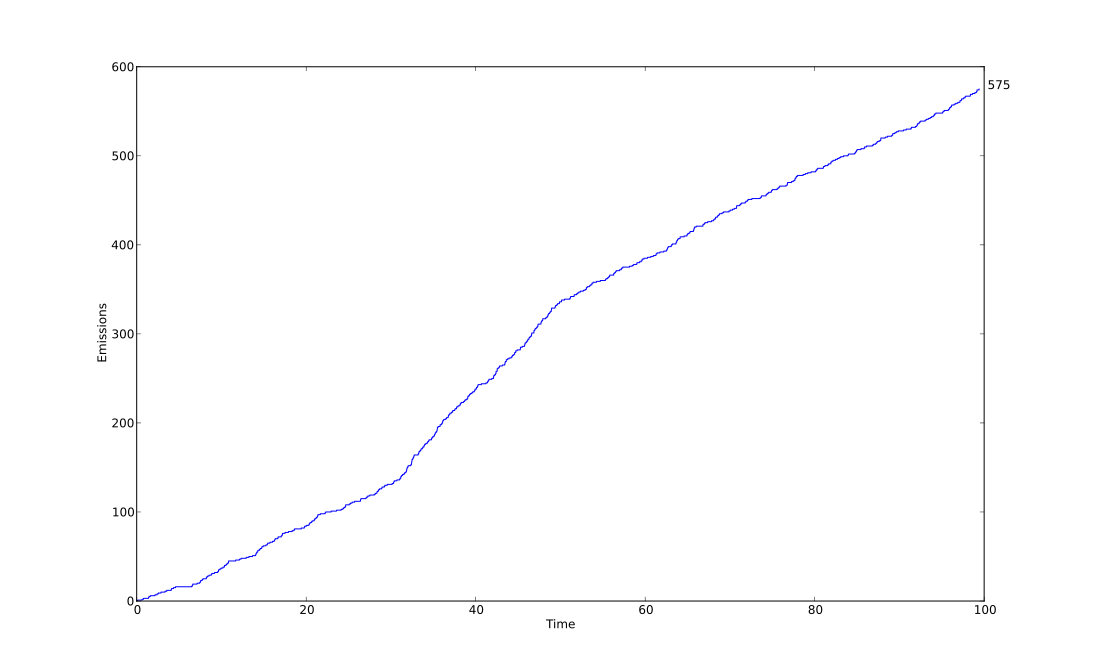
\includegraphics[width = 0.4\textwidth]{./images/trace_nonhom1.png}
    %\caption{A trace of an inhomogeneous Poisson process. Time flows along the x-axis, and the value on the y-axis shows the number of emissions seen thus far. A total of 575 emissions were observed.}
   \label{trace_nonhom1}
}
\subfloat[Its estimated rate]{
    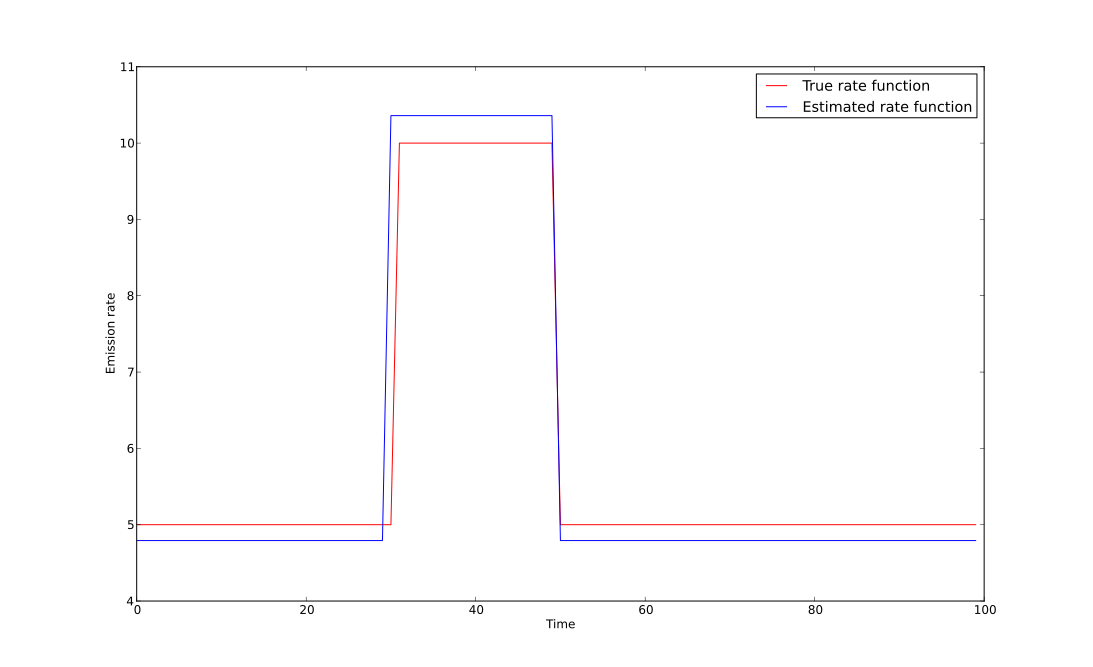
\includegraphics[width = 0.4\textwidth]{./images/fit_nonhom1.png}
    %\caption{An attempt to recover the rate function used to generate Figure \ref{trace_nonhom1}}
    \label{fit_nonhom1}
}
\caption{A realisation of a Poisson process, and its estimated rate.}

\end{figure}
We can fit a step function by observing multiple traces of these Poisson processes, taking the differences between emission times, then attempting to cluster them with the k-means algorithm \cite{kmeans}. Other approaches are possible, but because of how a step function can approximate an arbitrary function, and how easy it is to find implementations of k-means, these will suffice as an early heuristic. The average number of emissions per realisation is the integral of the rate with respect to time over the time interval for which we observe, i.e. if $N$ is the number of observed emissions in a single realisation,

$$
\mathbb{E}(N) = \int^{100}_0 \bm{\lambda}(t) \; dt = 600
$$

So if we simulate 6 realisations we'll observe roughly $3600$ emissions, a little more than our real data set. It's possible to attempt to fit this function with less data, but more data will give a more accurate result. Fitting a function to these gives us the results from Figure \ref{fit_nonhom1}. Eyeballing this, we see that it's not a terrible fit in this first attempt, but if we try a more complex rate function, a situation similar to Figure \ref{fit_nonhom2} happens. The estimations are well off the mark. We could instead attempt to fit a polynomial function with maximum likelihood or least squares or similar, but this requires more parameters, and completely ignores bursts. These bursts occur at random times throughout the day, and last for random lengths of time, but they all take on the same form. We need some randomness to our step function to allow for these bursts.

Clearly, a different approach is needed.

\begin{figure}[h]
\centering
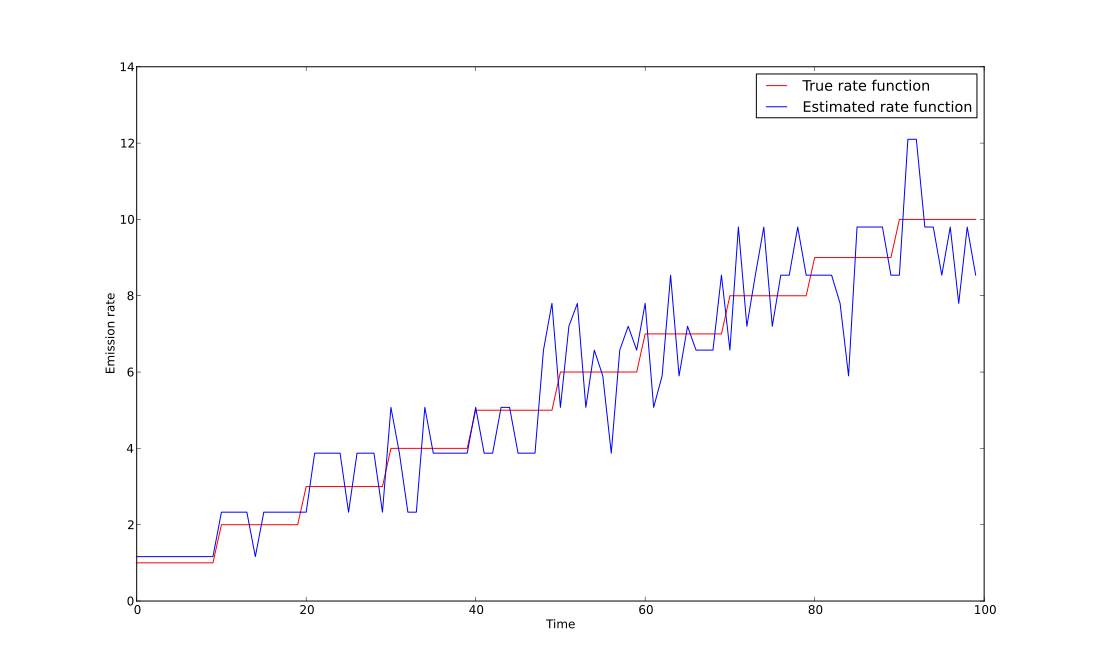
\includegraphics[width = 0.5\textwidth]{./images/fit_nonhom2.png}
\caption{A slightly more complex rate function, whose estimation barely resembles the original}
\label{fit_nonhom2}
\end{figure}

\clearpage

\section{Fitting a Markov-Modulated Poisson Process}

An MMPP seems ideal then, capturing the simplicity of a step function, and letting us model the idea of randomly distributed bursts throughout a day. Indeed, several authors have postulated that such a model would be ideal for simulating such data \cite{mmpp1}\cite{mmpp2}\cite{mmpp3}, but there have so far been no actual quantifiable studies of its relevance. This could be for a number of reasons, partially due to the lack of algorithms, but also possibly because these studies focus on somewhat smaller data sets. The Twitter user in this study is hugely active, yielding a vast quantity of data to fit, and making the true quality of the model all the clearer.

Fitting a Hidden Markov Model of any kind relies on two main algorithms, Baum-Welch \cite{baumwelch} and Viterbi \cite{viterbi}. The Baum-Welch algorithm is an expectation-maximisation algorithm for estimating the transition probabilities/rates and the emission probabilities, given a set of possible emissions, a number of states to fit and an observed sequence of emissions. The algorithm runs iteratively over the observed data, incrementally increasing the likelihood of the estimated model given the observations, and as such it needs an artificially defined stopping condition. In this project, we'll either use some fixed number of iterations, or stop when the log-likelihood increases by less than $10^{-6}$ between some pair of iterations, at which point we say that the model has converged sufficiently. Viterbi will take an observed sequence of emissions and the parameters of an HMM, usually those estimated by Baum-Welch, and produce the most likely state in which each of these emissions happened. The efficacy of these algorithms hinges on knowing the number of states, an issue which will be discussed later.

The HiddenMarkov package hosted on CRAN \cite{hiddenmarkov} is the only easily-accessible Hidden Markov Model package which supports the Markov Modulated Poisson Process, but does not contain any implementation of the Viterbi algorithm, and no implementation of Viterbi for the MMPP can be easily found. We have two ways of working around this, either write our own or discretise the process.

Since the times between emissions in an MMPP are usually exponentially distributed, we could work in discrete time by letting $y_t$ be the time between the $t^{th}$ and $(t+1)^{th}$ emissions, though this sacrifices some information. We no longer consider the possibility of making multiple transitions between emissions, and ignore the intrinsic link between the times between emissions and the times between state transitions, but this model may also yield some useful results. We will try both of these approaches.

\subsection{A derivation of the classical Viterbi algorithm}

The Viterbi algorithm for a standard Discrete Time Hidden Markov Model relies on a known, finite observation space $Y$, a known or estimated distribution on $Y$ for each state $s$, $p_s$,  known or estimated transition probabilities $\pi_{i,j}$, and known or estimated initial probabilities for each state $s$, $\delta_s$. The goal is, given a sequence of $N$ observations $(y_i)_{i \in [N]}$, $y_i \in Y$, to find the sequence of states $(x_i)_{i \in [N]}$ satisfying

$$
\mathbf{x} = \argmax_{\widehat{\mathbf{x}} \in S^N} \pr(\mathbf{\widehat{x}} | \mathbf{y})
$$

We call $\mathbf{x}$ the Viterbi Path.

Let $V_{t,s}$ be the probability of the most probable state sequence responsible for the first $t$ observations which ends in state $s$, that is

$$
V_{t,s} = \max_{\mathbf{\widehat{x}} \in S^{t-1}} \pr \Big((\widehat{x}_1,\widehat{x}_2,...,\widehat{x}_{t-1},s) \Big| (y_1,...,y_t)\Big)
$$

We have that $V_{1,s}$ is the probability of both being in state $s$ at time 1 and seeing observation $y_1$ from state $s$. This gives us that

$$
V_{1,s} = \pr (y_1|x_1 = s)\pr(x_1=s)
$$

Recall that $\delta_s$ is the probability of being in state $s$ at time 1, i.e. $\pr(x_1=s)$, and that $p_s(y_1)$ is the probability of observing $y_1$ from state $s$, i.e. $\pr (y_1|x_1 = s)$. In practice, these won't be known, but estimates of them will be given by the Baum-Welch algorithm, so we will use their maximum-likelihood estimates to give us

$$
V_{1,s} = p_s(y_1)\delta_s
$$

Given $V_{\tau,s}$ for $\tau < t$, we can find $V_{t,s}$ by noting that the Markov Property implies a form of memorylessness. Given the present, the future is conditionally independent of the past. As such, we need only consider $V_{t-1,s}$ for each $s$, as well as our known parameters. 

The probability of the most likely path that leads us to state $s$ at time $t$ is given by the probability of the most likely path that led us to some state $s'$ at time $t-1$, and then jumped to $s$ at time $t$, and then emitted $y_t$ from state $s$. The probability of jumping from $s'$ to $s$ is $\pi_{s',s}$. The probability of emitting $y_t$ from state $s$ is $P_s(y_t)$. The probability of the most likely path that leads us to $s'$ at time $t-1$ is $V_{t-1,s'}$. Hence,

$$
V_{t,s} = p_s(y_t) \max_{s'\in S} (\pi_{s',s}V_{t-1,s'})
$$

Using this recurrence, we can find $V_{t,s} \forall t \in [N], s \in S$ by a standard dynamic programming algorithm.

From here, we can then work backwards to find the Viterbi path. $x_N = \argmax_{s \in S} V_{N,s}$ - the most likely final state is the state in which the path of maximum probability ends.

Let
 
$$
T_{t,s} = \argmax_{s'\in S}(\pi_{s',s}V_{t-1,s'}),
$$
i.e., $T_{t,s}$ is the state from which we are most likely to have come at time $t-1$ given that we are in state $s$ at time $t$, we can then see that $x_{t-1} = T_{x_t,t}$. Note the similarities in the definitions of $V$ and $T$ - both can be calculated simultaneously - $V$ is the maximum, $T$ is the argument that maximises. $T_{1,s}$ is never used, so need never be defined. 

Since we have an expression for $x_{t-1}$ in terms of $x_t$ and an expression for $x_T$, we can then recover $\mathbf{x}$, the Viterbi Path. Algorithm \ref{algvitdthmm} gives this in full.

\begin{algorithm}
\SetAlgoLined
\SetKwInOut{Input}{input}
\SetKwInOut{Output}{output}

\caption{The Viterbi Algorithm for DTHMMs}\label{algvitdthmm}
\KwData{$(S,\bm{\delta},\Pi,O,p)$, a DTHMM}
\Input{$\mathbf{y}$, an observed sequence of $N$ emissions, indexed from $1$ to $N$}
\Output{$\mathbf{x}$, the most likely sequence of states generating these emissions}

\Begin{
	\For{$s \in S$}{
		$V_{1,s} <- p_s(y_1)\delta_s$
	}
	\For{$t \leftarrow 2$ \KwTo $N$}{
		\For{$s \in S$}{
			$V_{t,s} <- p_s(y_t) \max_{s' \in S}(\pi_{s',s}V_{t-1,s'})$ \\
			$T_{t,s} <- \argmax_{s' \in S}(\pi_{s',s}V_{t-1,s'})$
		}
	}
	$x_T <- \argmax_{s' \in S}(V_{s',T})$\\
	\For{$t \leftarrow T$ \KwTo $2$}{
		$x_{t-1} <- T_{x_t,t}$
	}
	\KwRet{$\mathbf{x}$}
}
\end{algorithm}

This algorithm is only valid in discrete time. For the continuous time MMPP, modifications are necessary.

\subsection{A First Approximation of the Viterbi Algorithm for the Markov-Modulated Poisson Process}

Recall the dependencies for the DTHMM Viterbi Algorithm. We require knowledge of a finite $Y$, $p_s$ for each $s\in S$, and $\pi_{ij}$ for each pair of states $i,j$.

In an MMPP, we observe a Poisson Process of rate randomly varying between various known rates - the rates being our states. Let $S = \{\lambda_1,...,\lambda_m\}$. Our observations can be interpreted as exponential random variables of these rates. Let $\tau_0 = 0$, and $\tau_i$ be the time of the $i^{th}$ Poisson emission for $i \in [N]$. Let $y_i = \tau_i-\tau_{i-1}$ for $i \in [N]$. Given that the underlying CTMC was in state $\lambda_s$ at time $\tau_i$, we have that $y_i \sim \mathrm{Exp} (\lambda_s)$. From the properties of the generic CTMC, the probability that the process is in state $j$ at time $\tau_i$ given that it was in state $i$ at time $\tau_{i-1}$ is given by $(e^{Qy_i})_{\lambda_{i},\lambda_{j}}$. This gives a quasi-discretised model, where all jumps and emissions indeed happen in discrete time, but the transition probabilities acknowledge continuity. To ease notation, we'll write $(e^{Qy_i})_{\lambda_{i},\lambda_{j}}$ as $(e^{Qy_i})_{i,j}$, omitting the $\lambda$s.

The state space $S$ and transition rates $Q$ are estimated by the Baum Welch algorithm as before, so after running Baum Welch over an observed sequence of emissions, we can start to find the most likely state at each emission. Note that this ``Viterbi Path" is not the most likely sequence of state transitions, it is instead the most likely state in which the underlying CTMC resides at the time of each emission. 

Since our emissions are continuous, we don't have any notion of ``most probable" - if we model height continuously, the probability that I meet someone exactly 1.8m tall is the same as the probability that I meet someone exactly 18m tall, they're both 0, so instead we'll base our likelihood calculations off probability density, capturing the idea that, even though I don't know for certain that I'll meet one of the two, it's more likely for me to meet the 1.8m tall person.

We let $p_s(t)= \lambda_s e^{-t\lambda_s}$, the probability density of an Exponential random variable of rate $\lambda_s$ evaluated at $t$. Let $V_{t,s}$ be the probability density of the most likely path that leads us to emitting $y_t$ from state $s$. We have that

$$
V_{1,s} =  \delta_{s}p_s(y_1)
$$

The probability density of the most likely path that leads us to waiting for time $y_1$ before making an emission is given by the probability of starting in state $s$, multiplied by the probability density of waiting $y_1$ for an emission from state $s$. The memoryless property of a CTMC allows us to only consider $V_{t-1,s}$ when calculating $V_{t,s}$. We have that

$$
V_{t,s} = p_s(y_t) \max_{s'\in S} (V_{t-1,s'}(e^{Qy_t})_{s',s})
$$

The probability density of the most likely path that leads us to waiting for time $y_t$ between the $(t-1)^{th}$ and $t^{th}$ emissions in state $s$ is given by the probability density of the most likely path that takes us to state $s'$ for the $(t-1)^{th}$ emission, followed by jumping (along any arbitrary path) into state $s$ for emission $t$, multiplied by the probability density of emitting $y_t$ in state $s$.

From here, we can proceed as before. We define $T$ as before to record our most likely states at each transition, and work backwards to find $\mathbf{x}$, producing algorithm \ref{viterbi_mmpp}.

\begin{algorithm}
\SetAlgoLined
\SetKwInOut{Input}{input}
\SetKwInOut{Output}{output}

\caption{An Approximate Viterbi Algorithm for MMPPs}\label{viterbi_mmpp}
\KwData{$(S,\bm{\delta},Q,p)$, an MMPP}
\Input{$\mathbf{y}$, the absolute times of an observed sequence of $N$ emissions, indexed from $1$ to $N$}
\Output{$\mathbf{x}$, the most likely sequence of states in which the underlying CTMC resides for each emission in $\mathbf{y}$}

\Begin{
	\For{$t <- 2$ \KwTo $N$}{
		$\tau_{t-1} <- y_t-y_{t-1}$
	}
	$N <- N-1$
	\For{$s \in S$}{
		$V_{1,s} <- p_s(t_1)\delta_s$
	}
	\For{$t \leftarrow 2$ \KwTo $N$}{
		$A <- e^{Q\tau_t}$
		\For{$s \in S$}{
			$V_{t,s} <- p_s(\tau_t) \max_{s' \in S}(A_{s',s}V_{t-1,s'})$ \\
			$T_{t,s} <- \argmax_{s' \in S}(A_{s',s}V_{t-1,s'})$
		}
	}
	$x_N <- \argmax_{s' \in S}(V_{s',N})$\\
	\For{$t \leftarrow N$ \KwTo $2$}{
		$x_{t-1} <- T_{x_t,t}$
	}
	\KwRet{$\mathbf{x}$}
}
\end{algorithm}

The reason that this is an approximation is the fact that the algorithm assumes that either a jump happens instantaneously, or not at all -- we always evaluate $p_s(y_t)$, rather than $p_s(y_t-\tengt)$\footnote{\tengt -- tinco -- represents the voiceless alveolar stop in the Tengwar alphabet, as devised by JRR Tolkein. When dealing with time so frequently, we eventually run out of ways to write the letter t}, where $\tengt$ represents the time we wait for all the relevant transitions to occur. The times between state transitions are exponentially distributed, and we are dealing with the most likely outcomes. The most likely outcome of any exponential distribution is $0$ so, if the underlying CTMC jumps from one state to another, the most likely time for that jump to happen is immediately, so $\tengt = 0$. If multiple jumps happen, their individual times are exponentially distributed, but their sum does not have a mode of 0.

This first approximation is in fact very powerful. Approximating in this way assumes that multiple transitions between emissions are rare, alternatively  that emissions within each state are more frequent than transitions out of that state. The converse can be true -- when the tweeter is asleep, his emission rate is near 0, but he will have a positive transition rate into a more active state -- and in this case the algorithm will spot periods of inactivity as estimate them as being the inactive state. If there are multiple states with low rate emissions but high rate transitions between them, then we would expect to see very few emissions occurring on a path through these states, so arguably the information on the exact route through these states doesn't exist, and cannot be recovered by any algorithm.

As a final note, we can further refine the fitted model based on the results of the Viterbi algorithm by changing the estimated rate of each state to the observed rate of the emissions estimated to occur in that state. By the nature of these estimation algorithms, these results are likely to differ, and with a large sample size what we observe is usually closer to the truth than what we assert. In practice, if Baum Welch gives a good estimation of the underlying MC, the difference between the two is minor.

\subsection{Applying the Algorithm}

The algorithm was written in R and added to the pre-existing HiddenMarkov \cite{hiddenmarkov} package, which was then recompiled to be loaded into an R environment. A Python script was written to call into this library from a more convenient language using RPy2 \cite{rpy} which also allowed mathematical, statistical and visualisation functions to be loaded in from matplotlib \cite{matplotlib}, and SciPy \cite{scipy}.

As before, we first simulate a model, then see if we can recover it, reassuring ourselves that the Viterbi implementation is correct. The simulated model had the following parameters;

\begin{align*}
(\lambda_1,\lambda_2,\lambda_3) &= (0.01,0.5,2)\\
S &= \{\lambda_1,\lambda_2,\lambda_3\}\\
Q &= \bordermatrix{      & \lambda_1 & \lambda_2 & \lambda_3\cr
                \lambda_1 & -0.05 & 0.0166...  & 0.033... \cr
                \lambda_2 & 0.1  & -0.133... & 0.033... \cr
                \lambda_3 & 0.1  & 0.0166...  & -0.1166...\cr
			}\\
\bm{\delta} &= \left(0.33...,0.33...,0.33...\right)
\end{align*}

The expected course of an MMPP is somewhat harder to calculate, but 6,000 hours gave a similar number of emissions to the number of emissions in our data. The resulting emissions can be seen in Figure \ref{trace_mmpp1}.

\clearpage
\begin{figure}[h!]
\centering
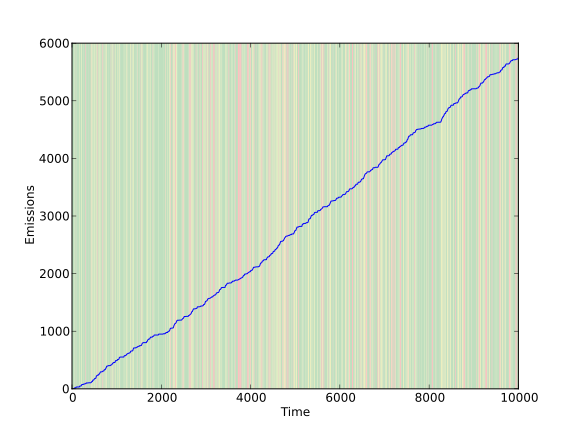
\includegraphics[width = 0.4\textwidth]{./images/trace_mmpp1.png}
\caption{A trace of an MMPP with the states shaded in colour \protect\footnotemark }
\label{trace_mmpp1}
\end{figure}
\footnotetext{Originally, all the diagrams in this document were vector graphics, but diagrams like this are so intricate that their vector versions can crash pdf renderers.}

Running the Baum-Welch algorithm over the realisation with a known state size of 3 for 208 iterations, at which the model converged sufficiently, gives us the following predictions, rounded to 2 significant Figures;

\begin{align*}
(\lambda_1,\lambda_2,\lambda_3) &= (0.0066,0.53,2.00)\\
S &= \{\lambda_1,\lambda_2,\lambda_3\}\\
Q &= \bordermatrix{      & \lambda_1 & \lambda_2 & \lambda_3\cr
                \lambda_1 & -0.061 & 0.022 & 0.039 \cr
                \lambda_2 & 0.10 & -0.14 & 0.053 \cr
                \lambda_3 & 0.094 & 0.020 & -0.11 \cr
			}\\
\bm{\delta} &= (1.00,0.00,0.00)
\end{align*}

On inspection, most these parameters give a reasonable approximation of the originals, but $\bm{\delta}$ seems to be well off the mark. The reason for this is fairly simple -- the simulated process had to start somewhere, and in this case it started in state 1. The algorithm was only given one realisation of the process, so to minimise the probability of error, it estimated that the underlying CTMC always starts in the state in which it was estimated to start. The initial distribution of the underlying CTMC isn't hugely relevant, however. We're interested in how the user tweets in the long term, and regardless of initial distribution this Markov Chain will reach an invariant distribution.

Running the modified Viterbi algorithm over the process gives the estimate in Figure \ref{fit_mmpp1}.

\begin{figure}[h!]
\centering
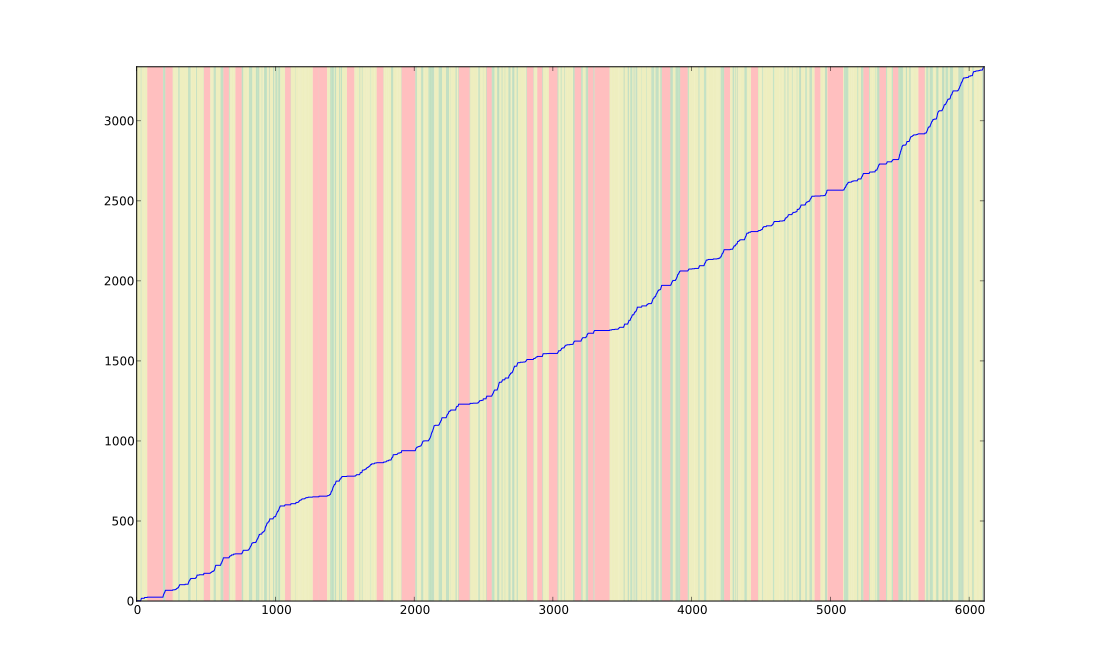
\includegraphics[width = 0.4\textwidth]{./images/fit_mmpp1.png}
\caption{The same process as Figure \ref{trace_mmpp1}, but with the shading to match estimated states, rather than actual states}
\label{fit_mmpp1}
\end{figure}

Comparing the estimated path to the original in a way that clearly displays the results seems daunting, but we can do this in what I find a fairly beautiful way by simply aligning the two traces along the same scale, rendering them as bitmaps, then taking the difference in the colours between the two images using GIMP \cite[eqn 8.15]{gimpdiff}. Any black pixels are locations where the original two images match perfectly, all others are mistakes. Stripping the top row of colours will show mistakes over time. Figure \ref{compare_mmpp1} is a black and white thresholded \cite{gimpthresh} version of the preceding, where all colours appear as white lines. The image is 91.2\% black so my estimated model matches the simulation 91.2\% of the time.

\begin{figure}[h!]
\centering
\includegraphics[width = 0.5\textwidth]{./images/compare_mmpp1_v2.png}
\caption{A comparison between the estimated state sequences of Figure \ref{fit_mmpp1} (top) and \ref{trace_mmpp1} (middle). Their image difference is shown at the bottom, with adjustments for clarity.}
\label{compare_mmpp1}
\end{figure}

Now that we've verified that our algorithms are capable of recovering known MMPPs to a high degree of accuracy, it's time to pump our data into it.

The data were preprocessed such that rather than recording exact times and dates of tweets, they instead recorded times since the beginning of the observation in hours at which each tweet occurred. This sequence was then fed into an MMPP data structure, over which BaumWelch and Viterbi were run based on the assumption of 3 states. This assumption is arbitrary, but serves as a nice starting point to generate some early results -- we'll address the problem of selecting the number of states later. The resulting model was as follows:
\begin{align*}
(\lambda_1,\lambda_2,\lambda_3) &= (0.0289,1.28,15.5)\\
S &= \{\lambda_1,\lambda_2,\lambda_3\}\\
Q &= \bordermatrix{      & \lambda_1 & \lambda_2 & \lambda_3\cr
                \lambda_1 & -0.123 & 0.120 & 0.004 \cr
                \lambda_2 & 0.441 & -1.09 & 0.648 \cr
                \lambda_3 & 0.00 & 5.25 & -5.25 \cr
			}\\
\bm{\delta} &= (1.00,0.00,0.00)
\end{align*}

With the states shaded in in the colours represented above, the transitions were as represented in Figure \ref{fit_mmpp2}.
\begin{figure}[h!]
\centering
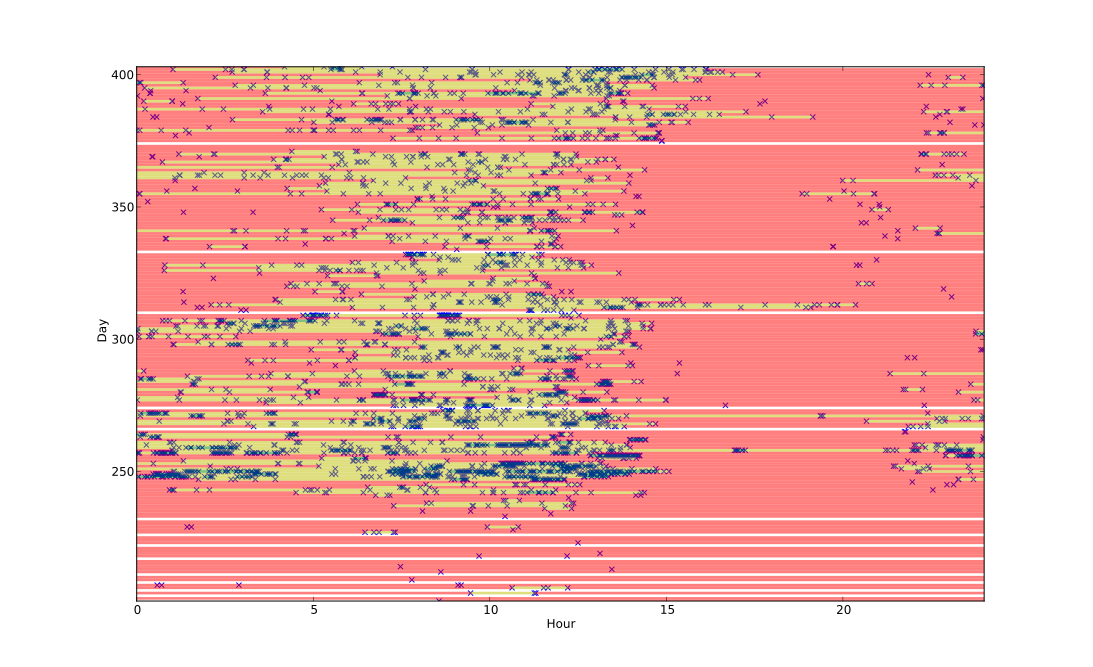
\includegraphics[width = 0.6\textwidth]{./images/fit_mmpp2.png}
\caption{The Twitter data, with predicted states shaded -- $\lambda_1$ in red, $\lambda_2$ in yellow, $\lambda_3$ in green. Since $\lambda_3$ is a burst state which, on average, only lasts for 12 minutes and contains several tweets, it can be difficult to see the green behind those tweets}
\label{fit_mmpp2}
\end{figure}
From this distance, we already see at least some kind of sensible behaviour - the user seems to have regular sleeping patterns, tweeting during the day and not tweeting at night-time. The three states correspond to intuitive states for a human to occupy -- in state $\lambda_1$ the user is asleep or otherwise away from the computer, tweeting on average once every 50 hours, but only staying there for 10 hours on average. In state $\lambda_2$, the user is awake, online, and going about his day as usual - as an active Twitter user he tweets about 1.3 times per hour. On average, every hour, the user will then either go to bed with probability $\approx 0.4$, or enter into a conversation with someone and produce a burst with probability $\approx 0.6$. This already seems a little odd, and shows the limitation of using a homogeneous model, we seem to be suggesting here that the user goes to bed on average every 1.5 hours, which doesn't fit our notions of how humans actually behave. Bursts are tweets produced at a rate of 15 per hour, or one every 4 minutes, and last around 12 minutes on average.

We can test whether this model gives an accurate representation of our data by performing a Kolmogorov-Smirnov (KS) \cite{mwkstest} test on the data for each state. This test takes the maximum difference in the cumulative distribution functions for the two data sets, and then compared to a critical value from the Kolmogorov distribution. This test generally requires a large data set to give meaningful results, but we certainly have one here. 

We take our null hypothesis to be that the emissions within each state follow an exponential distribution whose rate matches the observed rate. Running this test, we find, however, that they very much do not -- the p-values for each state were less than $2.2 \times 10^{-16}$ -- to say that this is low would be an understatement.

Whilst 3 states makes sense intuitively, there's no reason why this is definitely the case, so let's try different numbers of states. We can find the optimal number based on the Bayesian Information Criterion \cite{bic}. Given an estimated model, we can define the Bayesian Information Criterion, $BIC$, as

$$
BIC = -2 \ln L + k \ln n
$$

Where $\ln L$ is the log-likelihood of the fitted model, i.e. the natural logarithm of the probability of observing the data given that the model is correct, $k$ is the number of parameters fitted by model, and $n$ is the number of data points used to fit the model. Faced with the choice of two different models, we select the one with the lower BIC.

An MMPP of $|S|$ states has $k=|S|^2+|S| -1$ free parameters -- $Q$ contains $|S|^2$ elements, but each of the $|S|$ diagonal elements can be determined by the row on which it resides, we fit $s$ states, each of which is freely choosable, and $\delta$ has $|S|$ elements, one of which can be determined from the other $s-1$. The number of data points is one less than the number of tweets we've observed, and the log likelihood is returned by the Baum-Welch algorithm.

500 iterations of Baum-Welch were run over the data for varying numbers of states until the BIC stopped decreasing. This optimum occurred at 4 states with a BIC of 1470, described as follows:

\begin{align*}
(\lambda_1,\lambda_2,\lambda_3,\lambda_4) &= (0.0223,0.511,6.14,28.3)\\
S &= \{\lambda_1,\lambda_2,\lambda_3,\lambda_4\}\\
Q &= \bordermatrix{      & \lambda_1 & \lambda_2 & \lambda_3 & \lambda_4\cr
                \lambda_1 & -0.111 & 0.0950 & 0.0160 & 0.000 \cr
                \lambda_2 & 0.262  & -1.21  & 0.950  & 0.000 \cr
                \lambda_3 & 0.287  & 2.94   & -3.67  & 0.445 \cr
                \lambda_4 & 0.000  & 0.000  & 5.56   & -5.56 \cr
			}\\
\bm{\delta} &= (1.00,0.00,0.00,0.00)
\end{align*}

Fitted by the same methods, we see the results in Figure \ref{fit_mmpp3}.
\begin{figure}[h!]
\centering
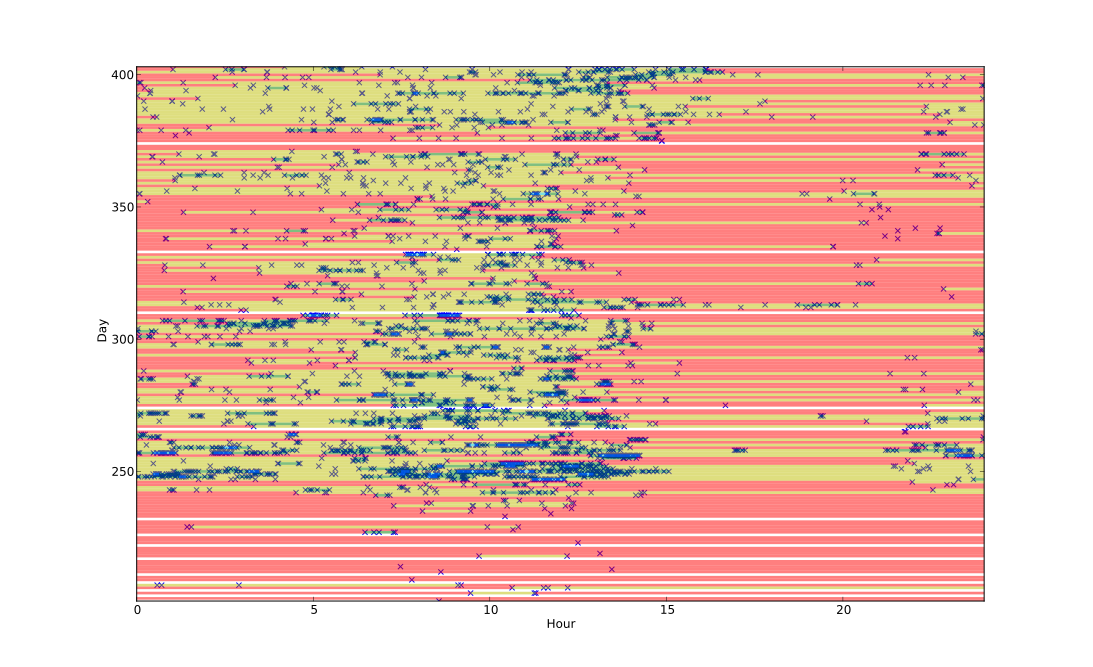
\includegraphics[width = 0.6\textwidth]{./images/fit_mmpp3.png}
\caption{The Twitter data, with predicted states shaded - $\lambda_1$ in red, $\lambda_2$ in yellow, $\lambda_3$ in green and $\lambda_4$ in cyan. As with $\lambda_3$ in Figure \ref{fit_mmpp1}, $\lambda_4$'s emissions can be difficult to see.}
\label{fit_mmpp3}
\end{figure}
Unfortunately, the Kolmogorov-Smirnov tests still fail - the greatest p-value for any state was $3.85 \times 10^{-6}$. Fitting more states would probably give a better fit, but due to the quadratic scaling it would also start sending the number of parameters up to absurd levels - the Bayesian Information Criterion would not improve. This is the best MMPP we can fit, and it still isn't very good.

\subsection{An Alternative Approach}

At this point, it is starting to seem like the tweeter does not follow an MMPP, but there is one last thing we can attempt in this vein. A Discrete Time Hidden Markov Model can still have a continuous observation space and all the previous methods will work. Rather than observing a series of times, we will instead observe a series of inter-arrival times, and look for any small number of states that lets us gather these times into the same exponential distribution. The results from such a model will be similar, but lose some information about how long our tweeter actually spends in each state. The crucial difference between the two is that in an MMPP emissions and transitions take place along the same timeline -- compare the Viterbi algorithms for both the MMPP and DTHMM, and note that the transition probabilities between a DTHMM's states do not depend on the observed emissions, whilst the transition probabilities in the MMPP version do.

So we go through the same procedure again - the intuitive 3 states didn't result in anything worthwhile, so we apply the BIC-based method again to arrive at an optimum of 5 states and a BIC of 1446, resulting in a DTHMM with the following parameters;

\begin{align*}
S &= \{1,2,3,4,5\}\\
(\lambda_1,\lambda_2,\lambda_3,\lambda_4,\lambda_5) &= (0.108, 1.18, 4.27, 14.8, 32.4)\\
\bm{\delta} &= (1,0,0,0,0)\\
\Pi &= 
\left(
    \begin{matrix}
    0.295 & 0.380 & 0.000 & 0.312 & 0.013 \\
    0.153 & 0.573 & 0.006 & 0.268 & 0.000 \\
    0.051 & 0.052 & 0.579 & 0.156 & 0.161 \\
    0.176 & 0.250 & 0.286 & 0.260 & 0.027 \\
    0.007 & 0.000 & 0.196 & 0.012 & 0.785
    \end{matrix}
\right)\\
Y &= \mathbb{R}^{+}\\
s \in S, y \in Y &=> p_s(y) = \lambda_s e^{-\lambda_sy}\\
\end{align*}

Which, when we add the Viterbi path to the plot, gives us Figure \ref{fit_dthmm1}. We perform some new KS tests to find one p-value of 0.03, and four others below $10^{-7}$. From this, we can definitively conclude that the data cannot be well-clustered into a small number of exponentially distributed subsets. We can then conclude that these data do not follow any kind of simple Poisson process, in spite of appearances.

\begin{figure}[h!]
\centering
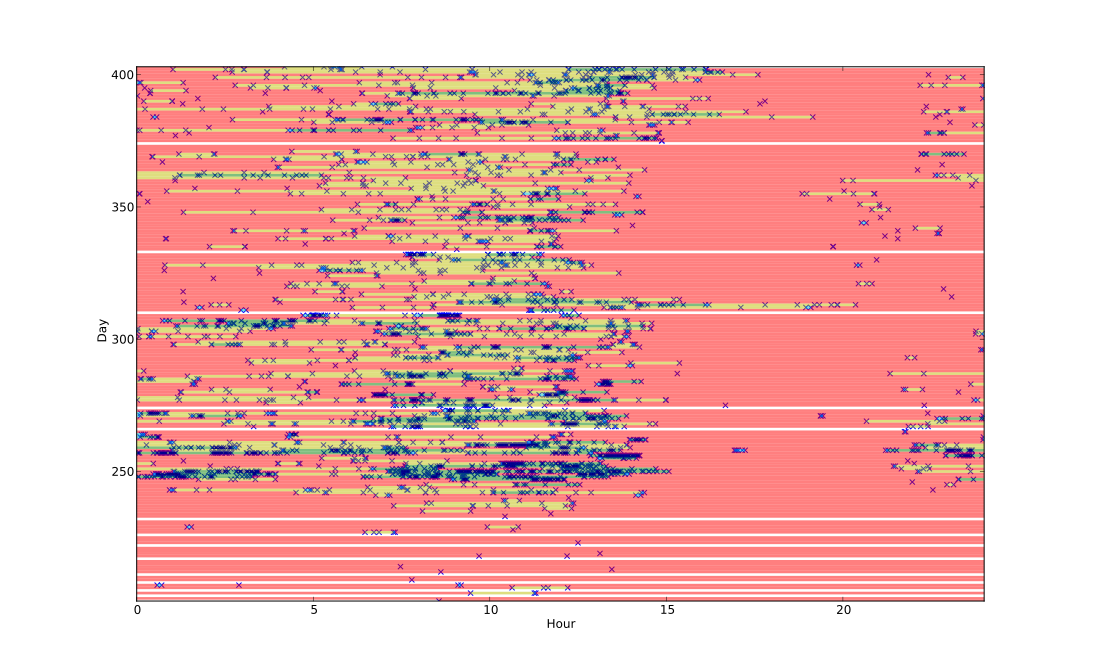
\includegraphics[width = 0.6\textwidth]{./images/fit_dthmm1.png}
\caption{The Twitter data, with predicted states shaded - $\lambda_1$ in red, $\lambda_2$ in yellow, $\lambda_3$ in green, $\lambda_4$ in cyan and $\lambda_5$ in black. Burst states are, as usual, very difficult to see.}
\label{fit_dthmm1}
\end{figure}

\section{A Diagnosis}

Whilst this gives a fairly strong negative result that this tweeter is not a Markov Modulated Poisson Process, it doesn't give any real explanation as to why. What went wrong? Inspecting the fitted models we see that the first few emissions don't quite fit in with the rest, but removing these anomalous results does little to the results of the Kolmogorov-Smirnov tests; they remain heavily negative in all cases.

Let's start looking at the emissions estimated to occur in each state. Since the DTHMM gave slightly better p-values, we'll use that as a jumping-off point.

And now, observing Figure \ref{densities_mmpp1} we see an issue. The fits are close, but the heads of the distributions are light and their tails heavy. What we really need is a distribution which will allow for this kind of skew, such as the lognormal distribution. If $X$ follows a lognormal distribution, then $\ln(X)$ follows a normal distribution \cite{mwlognormal}.

Summing lognormal distributions into a Markov Modulated Renewal Process in the same way that we sum exponential distributions into a Poisson process carries all manner of problems, however. The lognormal distribution is not memoryless nor is it modally 0, so the resulting processes within each state will be somewhat harder to fit, meaning that simple fitting algorithms like Baum-Welch and Viterbi require much more sophisticated modifications to work correctly in continuous time.

The algorithms for fitting a discrete model to the data using a DTHMM with lognormal emissions are, however, completely unchanged, so let's do that. We take the natural logarithm of all the inter-event times, fit multiple models and evaluate their BICs. Here, each state requires 2 parameters, a mean and a standard deviation, so the number of free parameters in an s-state model is now $s^2+2s-1$. We find that the optimal number of states is 3, and go ahead again with the KS tests, making minor corrections to the parameters for the estimated emissions within each state, resulting in p-values of 0.312, 0.156 and 0.420, and with densities shown in Figure \ref{densities_mmpp3}. At last, we have a model which is not rejected by the KS test, with the following parameters;

\begin{align*}
S &= \{1,2,3\}\\
(\mu_1, \mu_2, \mu_3) &= (-3.33, -1.33, 2.34)\\
(\sigma_1, \sigma_2, \sigma_3) &= (1.47, 1.86, 0.366)\\
\bm{\delta} &= (0,1,0)\\
\Pi &= 
\left(
	\begin{matrix}
     0.926 & 0.069 & 0.006 \\
     0.047 & 0.906 & 0.047 \\
     0.000 & 0.865 & 0.135
	\end{matrix}
\right)\\
Y &= \mathbb{R}\\
s \in S => p_s(y) &= \frac{\exp({-\frac{(y-\mu_s)^2}{2\sigma_s^2}})}{\sigma_s\sqrt{2\pi}}
\end{align*}

Given a sequence of emissions from this DTHMM, $\mathbf{y}$, the inter-arrival times are then $\bm{\tau}$ with $\tau_i = e^{y_i}$. Perhaps a little strangely, shading the states onto our graph as in Figure \ref{fit_dthmm2} gives a less obvious seasonality to the tweeter's behavior. We still have observable and highlighted bursts as well as some regularity to the user's sleeping patterns, but they're less obvious here than with the MMPP. More work would certainly throw up more results, perhaps this requires a continuous time model for such things to be seen, but regardless, this is a positive result for a problem whose solution has so far only been speculated upon, and which shows that these speculations are very likely to be wrong.
\clearpage

\begin{figure}
\centering
\subfloat{
    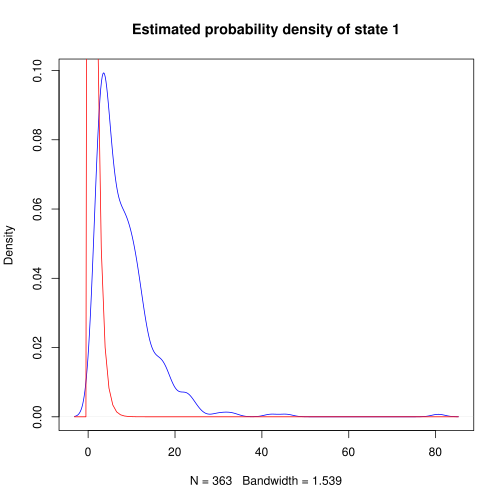
\includegraphics[width = 0.4 \textwidth]{./images/density_mmpp1_state1.png}
    \label{density_mmpp1_state1}
}
\subfloat{
    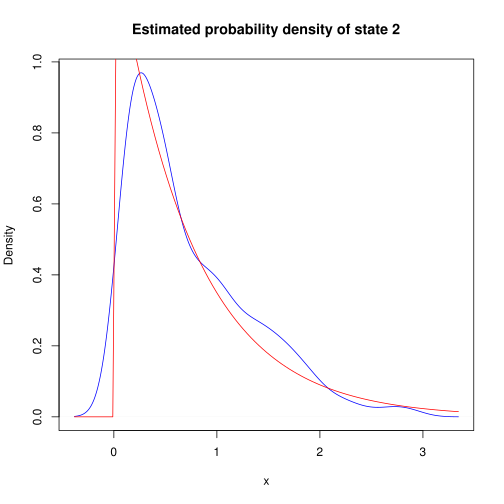
\includegraphics[width = 0.4 \textwidth]{./images/density_mmpp1_state2.png}
    \label{density_mmpp1_state2}
} \\

\subfloat{
    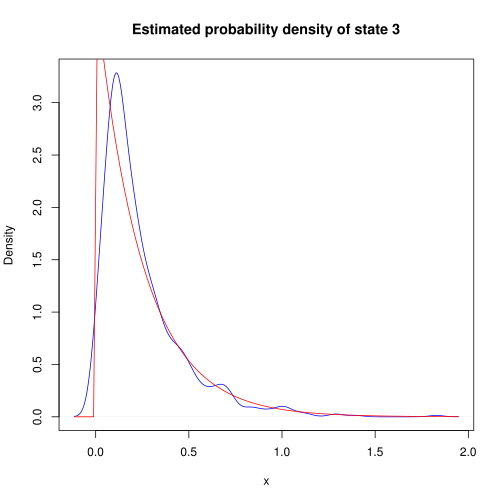
\includegraphics[width = 0.4 \textwidth]{./images/density_mmpp1_state3.png}
    \label{density_mmpp1_state3}
}
\subfloat{
    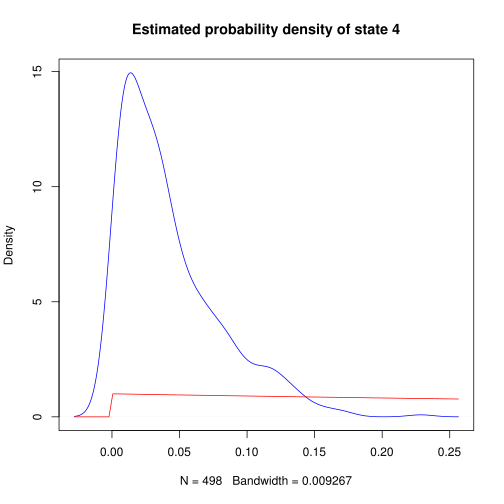
\includegraphics[width = 0.4 \textwidth]{./images/density_mmpp1_state4.png}
    \label{density_mmpp1_state4}
} \\
\subfloat{
    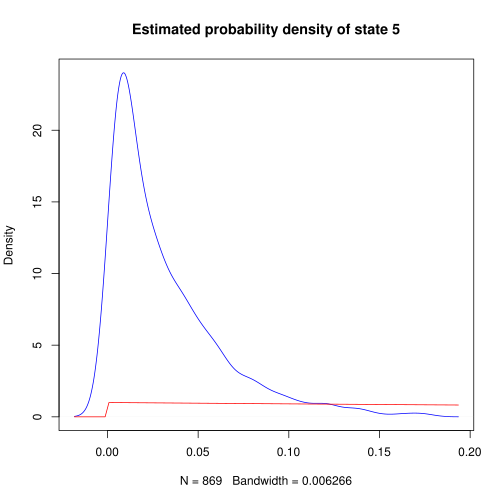
\includegraphics[width = 0.4 \textwidth]{./images/density_mmpp1_state5.png}
    \label{density_mmpp1_state5}
}
\caption{The estimated densities of emissions in each state (blue), alongside the actual density of an exponential random variable of rate equal to the rates of the observed emissions in that state}
\label{densities_mmpp1}
\end{figure}

\begin{figure}
\centering
\subfloat{
    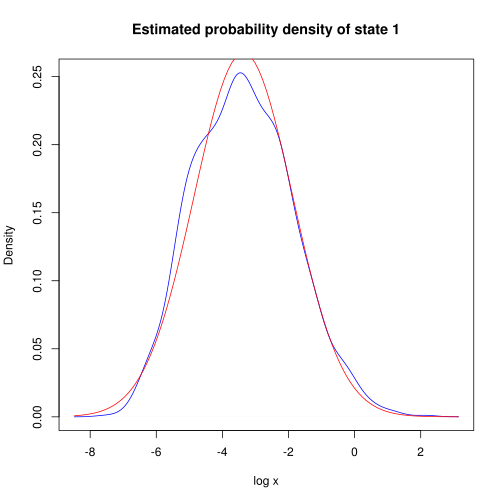
\includegraphics[width = 0.4 \textwidth]{./images/density_mmpp3_state1.png}
    \label{density_mmpp3_state1}
}
\subfloat{
    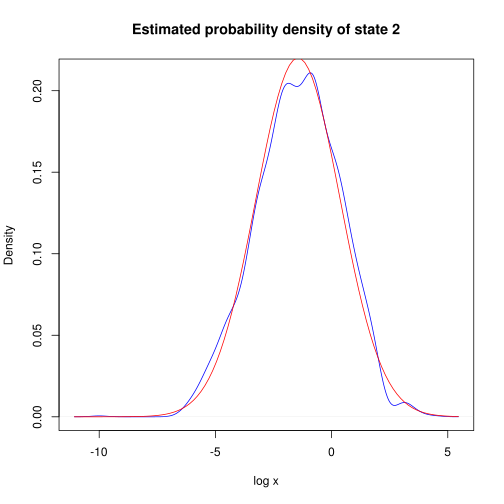
\includegraphics[width = 0.4 \textwidth]{./images/density_mmpp3_state2.png}
    \label{density_mmpp3_state2}
} \\

\subfloat{
    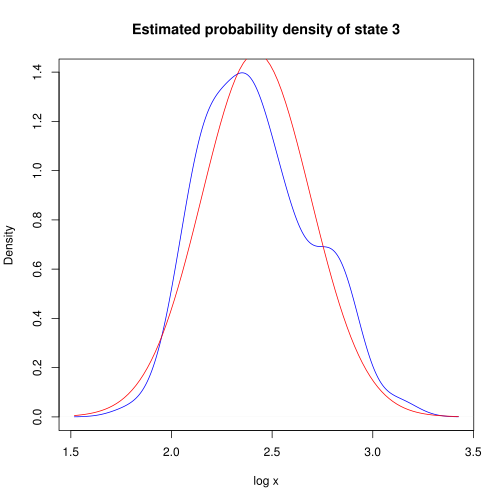
\includegraphics[width = 0.4 \textwidth]{./images/density_mmpp3_state3.png}
    \label{density_mmpp3_state3}
}
\caption{The estimated densities of the logarithms of emissions in each state (blue), alongside the actual density of a normal random variable of mean and variance equal to those of the logarithms of the observed emissions in that state}
\label{densities_mmpp3}
\end{figure}

\begin{figure}
\centering
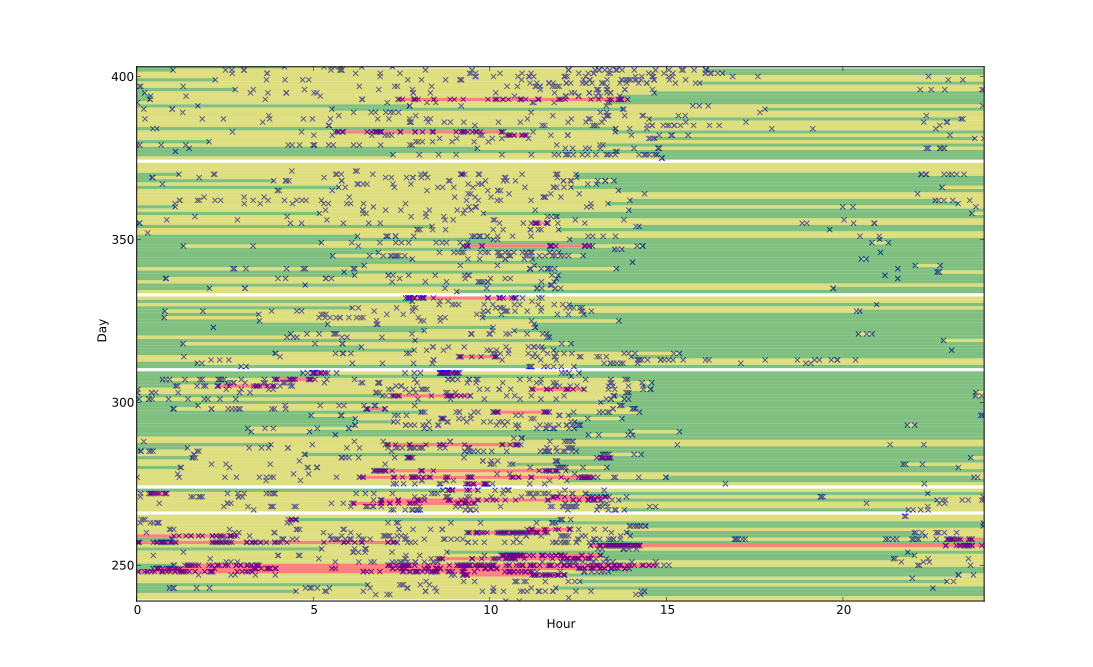
\includegraphics[width = \textwidth]{./images/fit_dthmm2.png}
\caption{The state transitions estimated by Viterbi for a DTHMM with lognormal emissions, state 1 in red, 2 in yellow, 3 in green}
\label{fit_dthmm2}
\end{figure}

